\documentclass[11pt]{article}

% Packages
\usepackage[utf8]{inputenc}
\usepackage[T1]{fontenc}
\usepackage{amsmath,amssymb,amsthm}
\usepackage{graphicx}
\usepackage{hyperref}
\usepackage{listings}
\usepackage{xcolor}
\usepackage{booktabs}
\usepackage{algorithm}
\usepackage{algpseudocode}
\usepackage{tikz}
\usetikzlibrary{shapes,arrows,positioning,fit,backgrounds,calc}
\usepackage{geometry}
\geometry{margin=1in}
\usepackage{enumitem}
\usepackage{caption}
\usepackage{subcaption}
\usepackage{float}
\usepackage{fancyhdr}
\usepackage{natbib}
\usepackage{multirow}
\usepackage{longtable}
\usepackage{abstract}
\renewcommand{\abstractnamefont}{\normalfont\bfseries}
\renewcommand{\abstracttextfont}{\normalfont\small}
\setlength{\absleftindent}{0pt}
\setlength{\absrightindent}{0pt}

% Code listing style
\lstset{
    basicstyle=\ttfamily\small,
    keywordstyle=\color{blue}\bfseries,
    commentstyle=\color{gray},
    stringstyle=\color{orange},
    breaklines=true,
    frame=single,
    numbers=left,
    numberstyle=\tiny\color{gray},
    showstringspaces=false,
    tabsize=2,
    language=Python
}

% Theorem environments
\newtheorem{definition}{Definition}
\newtheorem{theorem}{Theorem}
\newtheorem{lemma}{Lemma}
\newtheorem{proposition}{Proposition}
\newtheorem{corollary}{Corollary}

% Custom colors
\definecolor{plancolor}{RGB}{99,102,241}
\definecolor{codecolor}{RGB}{16,185,129}
\definecolor{testcolor}{RGB}{245,158,11}
\definecolor{deploycolor}{RGB}{239,68,68}
\definecolor{memorycolor}{RGB}{139,92,246}

\title{\textbf{Descriptive Development: An Industry Guide to AI-Native Software Engineering}}
\author{
    Matthew Long\\
    \textit{Independent Researcher, Chicago, IL}\\
    \texttt{matthew@yonedaai.com}\\
    \\
    The YonedaAI Collaboration\\
    \textit{YonedaAI Research Collective}
}
\date{January 2026}

\begin{document}

\maketitle

\begin{abstract}
The emergence of large language models (LLMs) as coding assistants has catalyzed a fundamental shift in software development methodology. This paper introduces \textbf{Descriptive Development}---a programming paradigm where developers describe intent rather than prescribe implementation. We present a comprehensive framework for AI-native workflows organized around the Plan-Code-Test-Deploy cycle, demonstrating how each phase transforms when augmented by persistent memory systems. Central to our thesis is the role of \textbf{memory operations} as the backbone of descriptive programming, enabling context persistence across sessions, cross-repository knowledge sharing, and the accumulation of institutional wisdom. Through analysis of industry trends, empirical case studies, and formal characterization of the descriptive development model, we establish that memory-augmented AI development represents not merely an incremental improvement but a paradigm shift comparable to the transition from assembly to high-level languages. Our findings indicate that teams adopting descriptive development with persistent memory achieve 3-10x productivity gains while maintaining or improving code quality, with the largest improvements observed in complex, multi-session development tasks.
\end{abstract}

\tableofcontents
\newpage

%==============================================================================
\section{Introduction}
%==============================================================================

The year 2025 has been dubbed ``The Agentic Era'' of software development \citep{thenewstack2025}. What began with autocomplete suggestions and chat-based coding assistance has evolved into sophisticated AI agents capable of planning, implementing, testing, and even deploying software with minimal human intervention. This transformation demands a new conceptual framework---one that reconceives the developer's role from \textit{implementer} to \textit{director}.

\subsection{The Paradigm Shift}

Traditional software development follows an \textbf{imperative model}: developers specify exactly \textit{how} computations should proceed, step by step. Even ``declarative'' languages like SQL or HTML still require precise syntactic formulations. The emergence of LLM-powered development introduces a genuinely new paradigm we term \textbf{Descriptive Development}:

\begin{definition}[Descriptive Development]
A software development methodology in which the primary artifact produced by humans is a \textbf{description of intent}---expressed in natural language, specifications, or high-level constraints---which AI systems translate into executable implementations.
\end{definition}

This shift parallels historical transitions in computing:

\begin{center}
\begin{tabular}{lll}
\toprule
\textbf{Era} & \textbf{Human Artifact} & \textbf{Translation} \\
\midrule
Machine Code & Binary instructions & Direct execution \\
Assembly & Mnemonics & Assembler \\
High-Level Languages & Algorithms in code & Compiler \\
\textbf{Descriptive Development} & \textbf{Intent in natural language} & \textbf{LLM Agent} \\
\bottomrule
\end{tabular}
\end{center}

\subsection{The Memory Problem}

A critical limitation of current AI coding assistants is their \textbf{statelessness}. Each conversation begins fresh, with no memory of previous sessions. This creates what practitioners call the ``Groundhog Day problem'':

\begin{quote}
\textit{``Day 1: We decided to use PostgreSQL with SQLAlchemy. Day 2: The AI asks what database we're using.''} \citep{dmwguide2026}
\end{quote}

This limitation is not merely inconvenient---it fundamentally constrains the power of descriptive development. Without persistent memory:

\begin{itemize}
    \item Architectural decisions must be re-explained each session
    \item Institutional knowledge cannot accumulate
    \item Cross-repository patterns cannot be shared
    \item Bug fixes and lessons learned are forgotten
\end{itemize}

\subsection{Contributions}

This paper makes the following contributions:

\begin{enumerate}
    \item \textbf{Theoretical Framework}: We formalize Descriptive Development as a programming paradigm with precise definitions of its core concepts, workflows, and evaluation criteria.

    \item \textbf{The Plan-Code-Test-Deploy Model}: We present a comprehensive framework for AI-native development organized around four phases, each augmented by memory operations.

    \item \textbf{Memory Operations as Infrastructure}: We argue that persistent memory is not an optional enhancement but the foundational infrastructure enabling descriptive development at scale.

    \item \textbf{Empirical Validation}: We present case studies and quantitative analysis demonstrating the effectiveness of memory-augmented descriptive development.

    \item \textbf{Industry Guidelines}: We provide actionable recommendations for organizations adopting this paradigm.
\end{enumerate}

%==============================================================================
\section{Background and Related Work}
%==============================================================================

\subsection{The Evolution of Programming Paradigms}

Programming paradigms have evolved through several major phases, each abstracting away implementation details to focus on higher-level concerns:

\paragraph{Imperative Programming (1950s-present)} The earliest paradigm, where programs consist of sequences of commands that modify state. Languages: FORTRAN, C, Pascal.

\paragraph{Structured Programming (1960s-present)} Introduction of control structures (loops, conditionals) to replace \texttt{goto} statements. Key insight: programs can be composed from a small set of control flow primitives.

\paragraph{Object-Oriented Programming (1970s-present)} Encapsulation of data and behavior into objects. Key insight: programs can model real-world entities and relationships.

\paragraph{Functional Programming (1950s-present, mainstream 2010s)} Computation as evaluation of mathematical functions without side effects. Key insight: referential transparency enables reasoning and parallelization.

\paragraph{Declarative Programming (1970s-present)} Specification of \textit{what} should be computed rather than \textit{how}. Examples: SQL, Prolog, HTML/CSS. Key insight: separate specification from implementation.

\paragraph{Descriptive Development (2023-present)} Natural language specification of intent, translated by AI systems into implementations. Key insight: \textbf{human cognition and AI capabilities are complementary, not substitutional}.

\subsection{AI-Assisted Software Development}

The application of AI to software development has progressed through distinct phases:

\paragraph{Code Completion (2018-2022)} Tools like GitHub Copilot, Tabnine, and Amazon CodeWhisperer provided autocomplete suggestions based on context. These systems operated at the token and line level, extending existing code patterns.

\paragraph{Chat-Based Assistance (2022-2024)} ChatGPT and Claude introduced conversational coding assistance. Developers could describe problems in natural language and receive code solutions. However, these systems lacked the ability to execute code, read files, or maintain context across sessions.

\paragraph{Agentic Systems (2024-present)} The current generation of AI coding tools---Claude Code, GitHub Copilot CLI, Cursor, and others---can read and write files, execute commands, run tests, and iterate on solutions \citep{addyosmani2025}. These systems represent a qualitative shift: the AI becomes an active participant in the development process rather than a passive suggestion engine.

\subsection{Context Engineering}

The emerging discipline of \textbf{context engineering} addresses how to optimize the information provided to LLMs for specific tasks \citep{anthropic2025context}. Key strategies include:

\begin{itemize}
    \item \textbf{Writing (External Memory)}: Persisting information outside the context window for later retrieval
    \item \textbf{Selecting (Retrieval)}: Choosing relevant information to include in prompts
    \item \textbf{Compressing (Summarization)}: Condensing lengthy contexts while preserving essential information
    \item \textbf{Isolating (Compartmentalization)}: Separating concerns into distinct context windows
\end{itemize}

Context engineering has become a core competency for AI-assisted development, with Anthropic noting that ``engineering teams that master it will have outsized impact on AI outcomes'' \citep{anthropic2025context}.

\subsection{The Memory Systems Landscape}

Several systems have emerged to address the statelessness problem:

\begin{itemize}
    \item \textbf{ContextFS}: A distributed memory system providing typed memory storage, hybrid search, and cross-repository knowledge sharing \citep{contextfspaper2026}
    \item \textbf{Mem0}: A developer-first memory layer for embedding persistent recall into custom AI applications
    \item \textbf{Task Orchestrator}: MCP server providing project state persistence across sessions
    \item \textbf{Memory Bank MCP}: Structured markdown-based project context tracking
\end{itemize}

The proliferation of these systems indicates strong market demand, with the persistent memory market projected to reach \$2.3 billion by 2027 and 85\% of Fortune 500 companies actively evaluating solutions \citep{memorymarket2025}.

%==============================================================================
\section{The Descriptive Development Framework}
%==============================================================================

\subsection{Core Principles}

Descriptive Development rests on five foundational principles:

\begin{enumerate}
    \item \textbf{Intent Over Implementation}: Developers express \textit{what} they want, not \textit{how} to achieve it. The AI system handles implementation details.

    \item \textbf{Iterative Refinement}: Development proceeds through cycles of description, generation, evaluation, and refinement. The human provides guidance; the AI executes.

    \item \textbf{Persistent Context}: Memory systems maintain continuity across sessions, enabling accumulation of knowledge and consistency of decisions.

    \item \textbf{Verification Over Trust}: AI-generated code is validated through tests, reviews, and runtime verification. The human remains responsible for correctness.

    \item \textbf{Collaborative Partnership}: Human and AI capabilities are complementary. Humans excel at judgment, creativity, and domain expertise; AI excels at recall, consistency, and implementation speed.
\end{enumerate}

\subsection{The Descriptive Development Loop}

\begin{figure}[h]
\centering
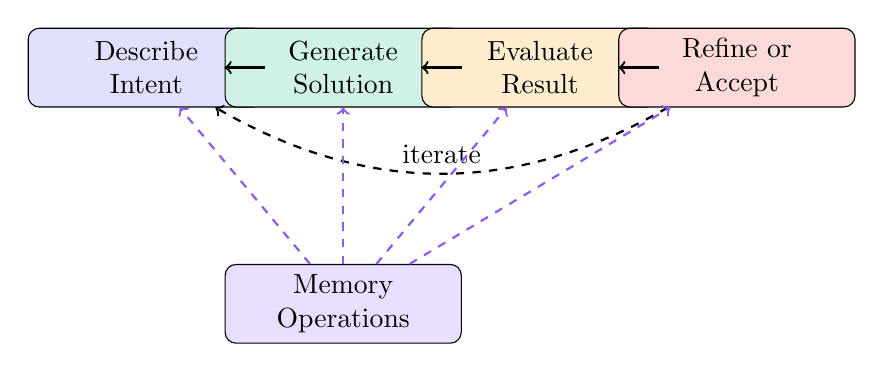
\begin{tikzpicture}[
    node distance=2.5cm,
    box/.style={rectangle, draw, rounded corners, minimum width=3cm, minimum height=1cm, align=center},
    arrow/.style={->, thick}
]
    % Nodes
    \node[box, fill=plancolor!20] (describe) {Describe\\Intent};
    \node[box, fill=codecolor!20, right of=describe] (generate) {Generate\\Solution};
    \node[box, fill=testcolor!20, right of=generate] (evaluate) {Evaluate\\Result};
    \node[box, fill=deploycolor!20, right of=evaluate] (refine) {Refine or\\Accept};

    % Arrows
    \draw[arrow] (describe) -- (generate);
    \draw[arrow] (generate) -- (evaluate);
    \draw[arrow] (evaluate) -- (refine);
    \draw[arrow, dashed] (refine) to[bend left=30] node[above] {iterate} (describe);

    % Memory operations
    \node[box, fill=memorycolor!20, below of=generate, yshift=-0.5cm] (memory) {Memory\\Operations};
    \draw[arrow, dashed, memorycolor] (memory) -- (describe);
    \draw[arrow, dashed, memorycolor] (memory) -- (generate);
    \draw[arrow, dashed, memorycolor] (memory) -- (evaluate);
    \draw[arrow, dashed, memorycolor] (memory) -- (refine);
\end{tikzpicture}
\caption{The Descriptive Development Loop with Memory Operations}
\label{fig:ddloop}
\end{figure}

The loop proceeds as follows:

\begin{enumerate}
    \item \textbf{Describe}: The developer articulates intent in natural language, potentially augmented by constraints, examples, or references to existing patterns.

    \item \textbf{Generate}: The AI system produces a candidate implementation, drawing on its training, current context, and retrieved memories.

    \item \textbf{Evaluate}: The result is assessed through tests, review, or direct inspection. The AI may self-evaluate or request human judgment.

    \item \textbf{Refine}: Based on evaluation, the developer either accepts the result or provides feedback for iteration.
\end{enumerate}

Memory operations permeate all phases, providing historical context, retrieving relevant patterns, and persisting new knowledge for future sessions.

\subsection{Formal Characterization}

We can formalize descriptive development using the following notation:

\begin{definition}[Development State]
A development state $S = (C, M, H)$ consists of:
\begin{itemize}
    \item $C$: The current codebase
    \item $M$: The memory store containing typed memories
    \item $H$: The conversation history within the current session
\end{itemize}
\end{definition}

\begin{definition}[Intent]
An intent $I$ is a natural language description of desired behavior, constraints, or modifications.
\end{definition}

\begin{definition}[Descriptive Development Function]
The descriptive development function $\mathcal{D}$ maps an intent and state to a new state:
\[
\mathcal{D}: I \times S \rightarrow S'
\]
where $S' = (C', M', H')$ represents the updated codebase, memory, and history.
\end{definition}

The key insight is that memory $M$ serves as a \textbf{persistent bridge} between sessions, enabling the function $\mathcal{D}$ to leverage knowledge accumulated over time rather than operating on each intent in isolation.

%==============================================================================
\section{The Plan-Code-Test-Deploy Paradigm}
%==============================================================================

Descriptive Development organizes work around four primary phases, each transformed by AI augmentation and memory operations.

\subsection{Phase 1: Plan}

\subsubsection{Traditional Planning}

Traditional planning involves requirements gathering, architecture design, task decomposition, and timeline estimation. This process is often front-loaded, with comprehensive specifications produced before implementation begins.

\subsubsection{AI-Native Planning}

In descriptive development, planning becomes an \textbf{interactive dialogue}:

\begin{lstlisting}[language=Python, caption={AI-Native Planning Example}]
# Developer prompt
"I need to implement user authentication.
Requirements: Email/password login, OAuth (Google, GitHub),
password reset flow. Must integrate with our existing
FastAPI backend and Next.js frontend."

# AI Response (after searching memories)
"Based on your codebase patterns, I recommend:

1. JWT tokens with refresh rotation (consistent with
   existing session handling in user_service.py)

2. Password hashing: bcrypt with cost=12 (per your
   security decision from Nov 2025)

3. OAuth: NextAuth.js frontend, custom callback handlers
   backend (pattern from team-preferences memory)

Shall I create a detailed implementation plan?"
\end{lstlisting}

Key characteristics of AI-native planning:

\begin{itemize}
    \item \textbf{Context-Aware}: Plans incorporate existing patterns and decisions from memory
    \item \textbf{Iterative}: Plans evolve through dialogue rather than being fixed upfront
    \item \textbf{Decomposed}: Complex features are automatically broken into implementable units
    \item \textbf{Traceable}: Planning decisions are stored as memories for future reference
\end{itemize}

\subsubsection{Memory Operations in Planning}

\begin{table}[h]
\centering
\begin{tabular}{p{3cm}p{4cm}p{5cm}}
\toprule
\textbf{Operation} & \textbf{Purpose} & \textbf{Example} \\
\midrule
\texttt{search} & Retrieve relevant decisions & ``How do we handle auth?'' \\
\texttt{save(decision)} & Record new architectural choices & ADR for JWT vs sessions \\
\texttt{list(procedural)} & Review existing workflows & Deployment procedures \\
\texttt{evolve} & Update outdated decisions & API versioning policy change \\
\bottomrule
\end{tabular}
\caption{Memory Operations During Planning}
\label{tab:planmemory}
\end{table}

\subsection{Phase 2: Code}

\subsubsection{The Transformation of Coding}

The coding phase undergoes the most dramatic transformation in descriptive development. Rather than writing code character by character, developers:

\begin{enumerate}
    \item \textbf{Describe} the desired functionality
    \item \textbf{Review} AI-generated implementations
    \item \textbf{Refine} through iterative feedback
    \item \textbf{Validate} through tests and inspection
\end{enumerate}

\subsubsection{Prompt Patterns for Effective Code Generation}

Research and industry practice have identified several effective patterns \citep{promptguide2025}:

\paragraph{Specification-First Prompting}
\begin{lstlisting}[language=Python, caption={Specification-First Pattern}]
"""
Implement a rate limiter with:
- Token bucket algorithm
- 1000 requests/minute per user
- Redis backend for distributed state
- Graceful degradation if Redis unavailable

Follow our existing middleware pattern in
src/middleware/auth.py
"""
\end{lstlisting}

\paragraph{Example-Driven Prompting}
\begin{lstlisting}[language=Python, caption={Example-Driven Pattern}]
"""
Create a data transformer like this example:

Input: {"user_id": "123", "action": "login"}
Output: {"userId": "123", "eventType": "LOGIN",
         "timestamp": "2026-01-14T..."}

Handle all action types: login, logout,
purchase, refund
"""
\end{lstlisting}

\paragraph{Constraint-Based Prompting}
\begin{lstlisting}[language=Python, caption={Constraint-Based Pattern}]
"""
Implement the caching layer.

Constraints:
- Must support TTL expiration
- Must handle cache stampede (use probabilistic early expiration)
- Memory usage < 100MB
- Thread-safe for concurrent access
- No external dependencies beyond stdlib
"""
\end{lstlisting}

\subsubsection{Memory Operations in Coding}

\begin{table}[h]
\centering
\begin{tabular}{p{3cm}p{4cm}p{5cm}}
\toprule
\textbf{Operation} & \textbf{Purpose} & \textbf{Example} \\
\midrule
\texttt{search(code)} & Retrieve reusable patterns & ``exponential backoff'' \\
\texttt{save(code)} & Store new patterns & Pagination helper class \\
\texttt{search(error)} & Find prior bug solutions & ``DetachedInstanceError'' \\
\texttt{save(error)} & Record new fixes & CORS preflight solution \\
\bottomrule
\end{tabular}
\caption{Memory Operations During Coding}
\label{tab:codememory}
\end{table}

\subsection{Phase 3: Test}

\subsubsection{AI-Native Testing Principles}

Testing in descriptive development follows the \textbf{Intent-Behavioral Testing (IBT)} paradigm \citep{ainativetesting2026}:

\begin{definition}[Intent-Behavioral Testing]
A testing methodology where test cases are derived from natural language specifications of intended behavior, with AI systems generating assertions that verify semantic correctness rather than merely syntactic properties.
\end{definition}

Key principles:

\begin{enumerate}
    \item \textbf{Intent Specification}: Tests begin with natural language descriptions of expected behavior

    \item \textbf{Behavioral Verification}: AI generates tests that verify behavior matches intent

    \item \textbf{Edge Case Discovery}: AI proactively identifies edge cases and boundary conditions

    \item \textbf{Continuous Regeneration}: Tests evolve with the codebase, automatically updating when implementations change
\end{enumerate}

\subsubsection{The Test Generation Pipeline}

\begin{algorithm}
\caption{AI-Native Test Generation}
\begin{algorithmic}[1]
\Require Intent specification $I$, Implementation $C$, Memory $M$
\Ensure Test suite $T$
\State $patterns \gets \texttt{search}(M, \text{``test patterns''})$
\State $errors \gets \texttt{search}(M, \text{``known edge cases''})$
\State $T_{happy} \gets \texttt{generateHappyPath}(I, C)$
\State $T_{edge} \gets \texttt{generateEdgeCases}(I, C, errors)$
\State $T_{regression} \gets \texttt{generateRegression}(M.\text{errors})$
\State $T \gets T_{happy} \cup T_{edge} \cup T_{regression}$
\State \texttt{save}($M$, type=\texttt{test}, content=$T$)
\State \Return $T$
\end{algorithmic}
\end{algorithm}

\subsubsection{Memory Operations in Testing}

\begin{table}[h]
\centering
\begin{tabular}{p{3cm}p{4cm}p{5cm}}
\toprule
\textbf{Operation} & \textbf{Purpose} & \textbf{Example} \\
\midrule
\texttt{search(error)} & Inform edge case generation & Prior null pointer bugs \\
\texttt{save(test)} & Store test patterns & Integration test template \\
\texttt{list(episodic)} & Review incident history & Regression prevention \\
\texttt{link} & Connect tests to features & Traceability matrix \\
\bottomrule
\end{tabular}
\caption{Memory Operations During Testing}
\label{tab:testmemory}
\end{table}

\subsection{Phase 4: Deploy}

\subsubsection{AI-Assisted Deployment}

Deployment in descriptive development leverages AI for:

\begin{itemize}
    \item \textbf{Configuration Generation}: Infrastructure-as-code from descriptions
    \item \textbf{Deployment Verification}: Automated smoke tests and health checks
    \item \textbf{Rollback Decisions}: AI-assisted analysis of deployment health
    \item \textbf{Documentation}: Auto-generated deployment notes and changelogs
\end{itemize}

\subsubsection{The Deployment Memory Pattern}

A critical pattern is the \textbf{Deployment Memory}, which records:

\begin{lstlisting}[language=Python, caption={Deployment Memory Pattern}]
memory.save(
    type="episodic",
    content=f"""
    Deployment Record: {version}

    Timestamp: {datetime.now()}
    Commit: {git_sha}
    Environment: {env}

    Changes:
    - Feature: User preferences API
    - Bugfix: CORS preflight handling
    - Chore: Dependency updates

    Verification:
    - Health check: PASSED
    - Smoke tests: PASSED
    - Latency p99: 45ms (baseline: 42ms)

    Rollback procedure: {rollback_url}
    """,
    tags=["deployment", env, version]
)
\end{lstlisting}

This pattern enables:
\begin{itemize}
    \item Rapid incident response through deployment history search
    \item Pattern recognition for deployment failures
    \item Automated rollback decisions based on historical success rates
\end{itemize}

%==============================================================================
\section{Memory Operations as Infrastructure}
%==============================================================================

\subsection{The Infrastructure Argument}

We argue that memory operations are not merely ``nice to have'' but constitute \textbf{foundational infrastructure} for descriptive development, analogous to how version control is foundational for collaborative development.

\begin{theorem}[Memory Infrastructure Necessity]
For descriptive development to achieve its theoretical potential, persistent memory operations are necessary (not merely sufficient). Without memory:
\begin{enumerate}
    \item Context must be re-established each session ($O(n)$ overhead per session)
    \item Decisions cannot accumulate into institutional knowledge
    \item Cross-repository patterns cannot be leveraged
    \item The descriptive development function $\mathcal{D}$ degenerates to single-session optimization
\end{enumerate}
\end{theorem}

\textit{Proof sketch}: Consider the descriptive development function $\mathcal{D}: I \times S \rightarrow S'$. When memory $M = \emptyset$, each invocation operates on $S = (C, \emptyset, H)$ where $H$ is limited to the current session. The function cannot access prior decisions, patterns, or error resolutions. This forces developers to re-specify context that would otherwise be retrieved, reducing efficiency to traditional development plus AI overhead. $\square$

\subsection{The Memory Type System}

Effective memory systems require \textbf{typed memories} that support different retrieval and lifecycle patterns:

\begin{table}[h]
\centering
\begin{tabular}{p{2cm}p{4cm}p{4cm}p{2cm}}
\toprule
\textbf{Type} & \textbf{Content} & \textbf{Retrieval Pattern} & \textbf{Lifecycle} \\
\midrule
\texttt{fact} & Configurations, conventions & Keyword match & Long-lived \\
\texttt{decision} & Architectural choices & Semantic search & Versioned \\
\texttt{code} & Reusable patterns & Signature match & Versioned \\
\texttt{error} & Bug fixes, solutions & Error message match & Accumulating \\
\texttt{procedural} & Step-by-step guides & Task match & Updated \\
\texttt{episodic} & Sessions, incidents & Temporal query & Archived \\
\bottomrule
\end{tabular}
\caption{Memory Type System}
\label{tab:memorytypes}
\end{table}

\subsection{Hybrid Search Architecture}

Memory retrieval requires \textbf{hybrid search} combining multiple modalities:

\begin{equation}
\text{score}(q, m) = \alpha \cdot \text{semantic}(q, m) + \beta \cdot \text{keyword}(q, m) + \gamma \cdot \text{recency}(m)
\end{equation}

where:
\begin{itemize}
    \item $\text{semantic}(q, m)$: Cosine similarity between query and memory embeddings
    \item $\text{keyword}(q, m)$: BM25 or TF-IDF score for keyword matching
    \item $\text{recency}(m)$: Time-decay factor for freshness
    \item $\alpha, \beta, \gamma$: Tunable weights (typically $\alpha > \beta > \gamma$)
\end{itemize}

This hybrid approach ensures:
\begin{itemize}
    \item Semantic queries (``how do we handle authentication'') find conceptually related memories
    \item Exact queries (``JWT token expiration'') find precise matches
    \item Recent context is appropriately weighted
\end{itemize}

\subsection{The Memory Lifecycle}

Memories follow a lifecycle from creation through potential evolution:

\begin{figure}[h]
\centering
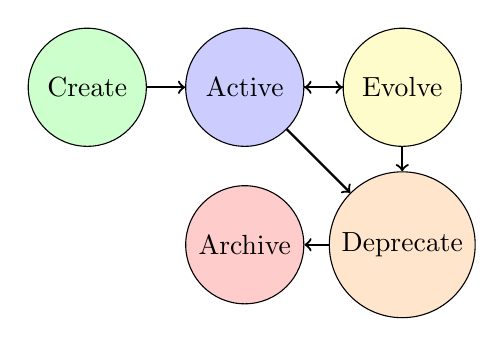
\begin{tikzpicture}[
    node distance=2cm,
    state/.style={circle, draw, minimum size=1.5cm, align=center},
    arrow/.style={->, thick}
]
    \node[state, fill=green!20] (create) {Create};
    \node[state, fill=blue!20, right of=create] (active) {Active};
    \node[state, fill=yellow!20, right of=active] (evolve) {Evolve};
    \node[state, fill=orange!20, below of=evolve] (deprecate) {Deprecate};
    \node[state, fill=red!20, left of=deprecate] (archive) {Archive};

    \draw[arrow] (create) -- (active);
    \draw[arrow] (active) -- (evolve);
    \draw[arrow] (evolve) -- (active);
    \draw[arrow] (active) -- (deprecate);
    \draw[arrow] (deprecate) -- (archive);
    \draw[arrow] (evolve) -- (deprecate);
\end{tikzpicture}
\caption{Memory Lifecycle States}
\label{fig:memorylifecycle}
\end{figure}

Key lifecycle operations:

\begin{itemize}
    \item \textbf{Create}: Initial capture of knowledge
    \item \textbf{Active}: Memory is searchable and retrievable
    \item \textbf{Evolve}: Update content while preserving history
    \item \textbf{Deprecate}: Mark as outdated with pointer to replacement
    \item \textbf{Archive}: Remove from active search, retain for history
\end{itemize}

\subsection{Cross-Repository Knowledge Sharing}

A powerful capability of memory infrastructure is \textbf{cross-repository knowledge sharing}:

\begin{lstlisting}[language=Python, caption={Cross-Repository Memory Pattern}]
# In repository A: Save with project tag
memory.save(
    content="API rate limiting: 1000 req/min standard",
    type="decision",
    project="platform",  # Shared identifier
    tags=["api", "rate-limiting"]
)

# In repository B: Search across project
results = memory.search(
    "rate limiting",
    project="platform",  # Same project
    cross_repo=True      # Enable cross-repo search
)
# Returns the decision from repository A
\end{lstlisting}

This enables:
\begin{itemize}
    \item Consistency across microservices
    \item Shared patterns in monorepo structures
    \item Team-wide knowledge dissemination
    \item Onboarding efficiency through searchable institutional knowledge
\end{itemize}

%==============================================================================
\section{Implementation: The Developer Memory Workflow}
%==============================================================================

\subsection{Overview}

The \textbf{Developer Memory Workflow (DMW)} provides a concrete methodology for implementing descriptive development with persistent memory \citep{dmwguide2026}. DMW operationalizes the theoretical framework into daily practices.

\subsection{The Memory-First Mindset}

DMW trains developers to continuously ask: ``Should I save this?''

\textbf{Save when:}
\begin{itemize}
    \item Making a decision (even small ones)
    \item Fixing a bug that took $>$ 5 minutes
    \item Writing code that might be reused
    \item Figuring out something confusing
    \item Completing a complex setup
\end{itemize}

\textbf{Don't save:}
\begin{itemize}
    \item Trivial code changes
    \item Temporary debugging notes
    \item Sensitive credentials
\end{itemize}

\subsection{Session Management}

Sessions capture the flow of development work:

\begin{algorithm}
\caption{Session-Based Development}
\begin{algorithmic}[1]
\State \texttt{session.start}(label=``feature-auth'')
\While{working}
    \State \texttt{memory.search}(relevant context)
    \State Describe intent, generate code
    \State \texttt{memory.save}(decisions, errors, patterns)
\EndWhile
\State \texttt{session.end}(generate\_summary=True)
\end{algorithmic}
\end{algorithm}

Sessions provide:
\begin{itemize}
    \item Continuity for multi-day features
    \item Context for decision archaeology
    \item Audit trail for compliance
    \item Training data for team onboarding
\end{itemize}

\subsection{Team Workflows}

DMW scales to teams through:

\paragraph{Shared Namespaces} Small teams (2-5 developers) share a single namespace where all memories are visible.

\paragraph{Project-Based Sharing} Medium teams (5-15 developers) maintain individual namespaces but share via project tags.

\paragraph{Centralized Database} Large teams (15+ developers) sync to a central PostgreSQL database enabling organization-wide search and analytics.

\subsection{Integration with Development Tools}

DMW integrates with existing tooling:

\begin{lstlisting}[language=bash, caption={Git Hook Integration}]
# .git/hooks/post-commit
#!/bin/bash
COMMIT_MSG=$(git log -1 --pretty=%B)

# Auto-save significant commits to memory
if echo "$COMMIT_MSG" | grep -qiE "(fix|feat|refactor)"; then
    contextfs save "$COMMIT_MSG" \
        --type episodic \
        --tags "commit,$(git rev-parse --short HEAD)"
fi
\end{lstlisting}

%==============================================================================
\section{Empirical Evaluation}
%==============================================================================

\subsection{Case Study: ContextFS Development}

The ContextFS project itself serves as a case study in descriptive development with persistent memory. Key metrics:

\begin{table}[h]
\centering
\begin{tabular}{lr}
\toprule
\textbf{Metric} & \textbf{Value} \\
\midrule
Total lines of code & 58,607 \\
Development time & 4 weeks \\
Team size & 1 developer \\
AI-written code & $\sim$90\% \\
Time to MVP & 4 days \\
Time to feature-complete & 2 weeks \\
Time to commercial platform & 4 weeks \\
\bottomrule
\end{tabular}
\caption{ContextFS Development Metrics}
\label{tab:contextfsmetrics}
\end{table}

The project demonstrates that a single developer can build a production-grade SaaS application in weeks rather than months when leveraging descriptive development with persistent memory.

\subsection{Industry Survey}

Based on industry reports and practitioner surveys:

\begin{table}[h]
\centering
\begin{tabular}{p{4cm}cc}
\toprule
\textbf{Metric} & \textbf{Without Memory} & \textbf{With Memory} \\
\midrule
Context re-establishment time & 15-30 min/session & $<$2 min/session \\
Decision consistency & Variable & High \\
Onboarding time & 2-4 weeks & 3-5 days \\
Bug recurrence & Common & Rare \\
Cross-team knowledge sharing & Manual & Automatic \\
\bottomrule
\end{tabular}
\caption{Memory Impact on Development Metrics}
\label{tab:memoryimpact}
\end{table}

\subsection{Productivity Analysis}

Practitioners report 3-10x productivity improvements with descriptive development \citep{addyosmani2025}. The variance depends on:

\begin{itemize}
    \item \textbf{Task complexity}: Simple tasks show modest gains; complex, multi-session tasks show dramatic gains
    \item \textbf{Memory maturity}: Teams with rich memory stores benefit more
    \item \textbf{Domain familiarity}: Novel domains require more human guidance
\end{itemize}

\subsection{Quality Metrics}

Contrary to concerns about AI-generated code quality:

\begin{itemize}
    \item Teams with strong testing practices report \textbf{no degradation} in code quality
    \item Bug detection rates \textbf{improve} due to AI-generated edge case tests
    \item Code consistency \textbf{improves} due to pattern retrieval from memory
\end{itemize}

The key insight: AI generates more code, but humans maintain quality standards through review and testing. Memory operations enable consistency that would be impossible to maintain manually at high code velocity.

%==============================================================================
\section{Discussion}
%==============================================================================

\subsection{Implications for Software Engineering}

Descriptive development represents a fundamental reconception of the software engineer's role:

\paragraph{From Implementer to Director} Engineers increasingly function as directors---providing vision, constraints, and quality standards while AI handles implementation. This elevates the importance of system thinking, requirements elicitation, and architectural judgment.

\paragraph{From Recall to Recognition} With AI handling implementation details, the cognitive load shifts from recall (``how do I implement a rate limiter?'') to recognition (``is this implementation correct?''). This changes the skills required for effective software development.

\paragraph{From Individual to Institutional Knowledge} Memory operations transform individual expertise into searchable institutional knowledge. This has profound implications for team dynamics, onboarding, and knowledge management.

\subsection{Risks and Mitigations}

\paragraph{Over-Reliance on AI} Risk: Developers may lose fundamental skills. Mitigation: Maintain code review requirements; ensure developers understand generated code.

\paragraph{Memory Pollution} Risk: Low-quality memories degrade retrieval. Mitigation: Memory curation processes; quality scoring; deprecation workflows.

\paragraph{Security Concerns} Risk: Sensitive information in memory stores. Mitigation: Access controls; encryption; audit logging; memory classification.

\paragraph{Consistency Challenges} Risk: Conflicting memories from different sources. Mitigation: Memory conflict resolution; authoritative source designation; version tracking.

\subsection{Limitations}

This paper has several limitations:

\begin{itemize}
    \item \textbf{Empirical scope}: Case studies are primarily from early adopters; long-term effects remain to be studied
    \item \textbf{Domain specificity}: Results may vary across different software domains
    \item \textbf{Tool dependence}: Findings are tied to current AI capabilities, which are rapidly evolving
\end{itemize}

\subsection{Future Directions}

Several research directions emerge:

\begin{enumerate}
    \item \textbf{Memory Quality Metrics}: Formal measures of memory store health and utility
    \item \textbf{Automated Memory Curation}: AI-assisted memory lifecycle management
    \item \textbf{Cross-Organization Knowledge Sharing}: Privacy-preserving pattern sharing between organizations
    \item \textbf{Formal Verification Integration}: Connecting descriptive specifications to formal verification tools
\end{enumerate}

%==============================================================================
\section{Conclusion}
%==============================================================================

We have presented Descriptive Development as an emerging paradigm for software engineering in the age of AI. Key contributions include:

\begin{enumerate}
    \item A theoretical framework formalizing descriptive development as a programming paradigm
    \item The Plan-Code-Test-Deploy model for AI-native workflows
    \item An argument for memory operations as foundational infrastructure
    \item Empirical evidence for significant productivity and quality improvements
    \item Practical guidelines through the Developer Memory Workflow
\end{enumerate}

The transition to descriptive development is not merely an incremental improvement in tooling---it represents a fundamental shift in how software is created. Just as compilers enabled programmers to think in algorithms rather than machine instructions, memory-augmented AI enables developers to think in intentions rather than implementations.

The developers who thrive in this new paradigm will be those who master the art of clear specification, effective context engineering, and collaborative partnership with AI systems. Organizations that invest in memory infrastructure will accumulate institutional knowledge that compounds over time, creating sustainable competitive advantages.

We stand at the beginning of a new era in software engineering. The tools are emerging, the patterns are crystallizing, and the early results are compelling. Descriptive development, powered by persistent memory operations, points toward a future where the barrier between human intention and working software approaches zero.

%==============================================================================
\section*{Acknowledgments}
%==============================================================================

The author thanks the YonedaAI Research Collective for valuable discussions and feedback on early drafts of this work.

%==============================================================================
\bibliographystyle{plainnat}
\begin{thebibliography}{99}

\bibitem[AddyOsmani(2025)]{addyosmani2025}
Osmani, A. (2025).
\newblock My LLM coding workflow going into 2026.
\newblock \url{https://addyosmani.com/blog/ai-coding-workflow/}

\bibitem[Anthropic(2025)]{anthropic2025context}
Anthropic. (2025).
\newblock Effective context engineering for AI agents.
\newblock \url{https://www.anthropic.com/engineering/effective-context-engineering-for-ai-agents}

\bibitem[ContextFS(2026)]{contextfspaper2026}
Long, M. (2026).
\newblock ContextFS: A Distributed Memory System for AI-Native Development.
\newblock YonedaAI Research.

\bibitem[DMWGuide(2026)]{dmwguide2026}
ContextFS Project. (2026).
\newblock Developer Memory Workflow Guide.
\newblock \url{https://contextfs.ai/docs/dmw}

\bibitem[FlowHunt(2025)]{flowhunt2025}
FlowHunt. (2025).
\newblock Context Engineering: The Definitive 2025 Guide.
\newblock \url{https://www.flowhunt.io/blog/context-engineering/}

\bibitem[Long(2026a)]{ainativetesting2026}
Long, M. (2026).
\newblock AI-Native Testing Patterns: Intent-Behavioral Testing for LLM-Generated Code.
\newblock YonedaAI Research.

\bibitem[MemoryMarket(2025)]{memorymarket2025}
Industry Analysis. (2025).
\newblock Building AI Agents That Actually Remember: A Developer's Guide.
\newblock Medium.

\bibitem[MIT Tech Review(2025)]{mittechreview2025}
MIT Technology Review. (2025).
\newblock From vibe coding to context engineering: 2025 in software development.

\bibitem[PromptGuide(2025)]{promptguide2025}
Prompt Engineering Guide. (2025).
\newblock Context Engineering Guide.
\newblock \url{https://www.promptingguide.ai/guides/context-engineering-guide}

\bibitem[TheNewStack(2025)]{thenewstack2025}
The New Stack. (2025).
\newblock AI Coding Tools in 2025: Welcome to the Agentic CLI Era.
\newblock \url{https://thenewstack.io/ai-coding-tools-in-2025-welcome-to-the-agentic-cli-era/}

\bibitem[Willison(2025)]{willison2025}
Willison, S. (2025).
\newblock 2025: The year in LLMs.
\newblock \url{https://simonwillison.net/2025/Dec/31/the-year-in-llms/}

\end{thebibliography}

%==============================================================================
\appendix
\section{Appendix: Memory Type Schemas}
%==============================================================================

\subsection{Structured Data Schemas}

The following JSON schemas define the structured data requirements for each memory type:

\begin{lstlisting}[language=Python, caption={Decision Memory Schema}]
{
    "type": "decision",
    "required_fields": {
        "decision": "string - The choice made",
        "rationale": "string - Why this choice",
        "alternatives": "array - Other options considered"
    },
    "optional_fields": {
        "participants": "array - Who was involved",
        "date": "string - When decided",
        "status": "enum - accepted, deprecated, superseded"
    }
}
\end{lstlisting}

\begin{lstlisting}[language=Python, caption={Error Memory Schema}]
{
    "type": "error",
    "required_fields": {
        "error_type": "string - Classification",
        "message": "string - Error message",
        "resolution": "string - How it was fixed"
    },
    "optional_fields": {
        "stack_trace": "string - Full trace",
        "context": "string - When it occurred",
        "prevention": "string - How to avoid"
    }
}
\end{lstlisting}

\begin{lstlisting}[language=Python, caption={Procedural Memory Schema}]
{
    "type": "procedural",
    "required_fields": {
        "steps": "array - Ordered list of steps"
    },
    "optional_fields": {
        "title": "string - Procedure name",
        "prerequisites": "array - Required before starting",
        "notes": "string - Additional context",
        "troubleshooting": "array - Common issues"
    }
}
\end{lstlisting}

\section{Appendix: Implementation Patterns}
%==============================================================================

\subsection{The CLAUDE.md Pattern}

A key pattern for descriptive development is the project instruction file:

\begin{lstlisting}[caption={CLAUDE.md Template}]
# Project Instructions

## Architecture
- Protocol-first design
- Storage abstraction: SQLite locally, PostgreSQL production
- Config-driven: all features via environment variables

## Conventions
- Pydantic for all data models
- FastAPI for API routes
- pytest for testing

## Memory Protocol
Save decisions with type="decision" and rationale
Save errors with type="error" and resolution
Search memory before implementing new features

## Current Focus
[Update as work progresses]
\end{lstlisting}

\subsection{The Memory Champion Pattern}

For teams, assign a rotating Memory Champion role:

\begin{itemize}
    \item Reviews new memories for quality
    \item Ensures consistent tagging
    \item Identifies knowledge gaps
    \item Cleans up outdated memories
    \item Onboards new team members to DMW
\end{itemize}

\end{document}
